\documentclass[sigconf, screen, review]{acmart}
% \documentclass[sigconf, screen]{acmart}
\citestyle{acmauthoryear}
\usepackage{xspace}
% \usepackage[abbreviations]{glossaries-extra}
% \usepackage[abbreviations]{glossaries}
\usepackage{glossaries}
\usepackage{amsmath}
\usepackage{mathtools}
\usepackage{wrapfig}
\usepackage{url}
\usepackage{xcolor, colortbl}
\usepackage[abbreviations]{glossaries-extra}

\definecolor{acmgreen}{RGB}{0,128,0}

\AtBeginDocument{%
  \providecommand\BibTeX{{%
    Bib\TeX}}}



\setcopyright{rightsretained}
\copyrightyear{2025}
\acmYear{2025}
\acmConference{SIGGRAPH}
\acmISBN{979-8-4007-1549-5/2025/08}


\newacronym{VAE}{VAE}{Variational Auto-Encoder}
\newacronym{INR}{INR}{Implicit Neural Representations}
\newacronym{PSNR}{PSNR}{Peak Signal-to-Noise Ratio}
\newacronym{SSIM}{SSIM}{Structural Similarity Index Measure}
\newacronym{3D}{3D}{Three-Dimensional}
\newacronym{MLP}{MLP}{Multi-Layer Perceptron}
\newacronym{CGH}{CGH}{Computer-Generated Holography}
\newacronym{CNN}{CNN}{Convolutional Neural Network}
\newabbreviation{DCT}{DCT}{Discrete Cosine Transform}

\global\long\def\CGH{\acrshort{CGH}\xspace}
\global\long\def\CNN{\acrshort{CNN}\xspace}
\global\long\def\VAE{\acrshort{VAE}\xspace}
\global\long\def\INR{\acrshort{INR}\xspace}
\global\long\def\PSNR{\acrshort{PSNR}\xspace}
\global\long\def\SSIM{\acrshort{SSIM}\xspace}
\global\long\def\TAESD{\textcolor{ColorTAESD}{\textbf{TAESD}}\xspace}
\global\long\def\MLP{\textcolor{ColorMLP}{\textbf{\acrshort{MLP}}}\xspace}
% \global\long\def\vanillaMLP{\textcolor{ColorMLP}{\textbf{vanilla MLP}}\xspace}
\global\long\def\SIREN{\textcolor{ColorSIREN}{\textbf{SIREN}}\xspace}
\global\long\def\FILMSIREN{\textcolor{ColorFILMSIREN}{\textbf{FilmSIREN}}\xspace}

\global\long\def\DCT{\gls{DCT}\xspace}

\newcommand{\etal}{~et al.\@\xspace}
\newcommand{\etc}{etc.\@\xspace}
\newcommand{\eg}{e.g.\@\xspace}
\newcommand{\Eg}{E.g.\@\xspace}
\newcommand{\ie}{i.e.\@\xspace}
\newcommand{\Ie}{I.e.\@\xspace}
\newcommand{\Fig}{Fig.\@\xspace}
\newcommand{\fig}{Fig.\@\xspace}
\newcommand{\eq}{Eq.\@\xspace}
\newcommand{\refSec}[1]{Sec.~\ref{sec:#1}}
\newcommand{\refSupSec}[1]{Sec.~\ref{#1}}
\newcommand{\refFig}[1]{Fig.~\ref{fig:#1}}
\newcommand{\refFigFull}[1]{Figure~\ref{fig:#1}}
\newcommand{\refEq}[1]{Eq.~(\ref{eq:#1})}
\newcommand{\refTbl}[1]{Tbl.~\ref{tbl:#1}}
\newcommand{\refObj}[1]{Objective~\ref{obj:#1}}
\newcommand\paraspace{-2.0mm}

\definecolor{ColorMLP}{rgb}{0.8470588235294118, 0.10588235294117647, 0.3764705882352941}
\definecolor{ColorSIREN}{rgb}{0.11764705882352941, 0.5333333333333333, 0.8980392156862745}
\definecolor{ColorFILMSIREN}{rgb}{1, 0.7568627450980392, 0.027450980392156862}
\definecolor{ColorTAESD}{rgb}{0, 0.30196078431372547, 0.25098039215686274}

\newcommand{\phaseonlyhologram}{P\xspace}
\newcommand{\wavelengths}{\lambda\xspace}
\newcommand{\pixelpitch}{px\xspace}
\newcommand{\bottleneck}{\alpha\xspace}

\newcommand{\colorOutputField}[1]{\textcolor{ColorOutputField}{#1}}

\settopmatter{authorsperrow=4}

\begin{document}

\title{Assessing Learned Models for Phase-only Hologram Compression}

\author{Zicong Peng}
\affiliation{%
  \institution{KOC University}
  \city{Istanbul}
  \country{tr}
}
\email{zpeng25@ku.edu.tr}


\author{Kaan Akşit}
\affiliation{%
  \institution{University College London}
  \city{London}
  \country{UK}
}
\email{k.aksit@ucl.ac.uk}

\renewcommand{\shortauthors}{Peng et al.}


\begin{abstract}
   Based on what I have learnt so far, I would like to systematically organize 
   the papers, researches, classes, books that I found and explored. This paper
   will try to collect the recent Models, perspectives and theories in good conference or journals.
   In addition, it is the note to record my idea and question to improve my understanding and probably prove my directions
\end{abstract}

\begin{CCSXML}
<ccs2012>
   <concept>
       <concept_id>10010147.10010371.10010395</concept_id>
       <concept_desc>Computing methodologies~Image compression</concept_desc>
       <concept_significance>500</concept_significance>
       </concept>
   <concept>
       <concept_id>10003752.10003809.10010031.10002975</concept_id>
       <concept_desc>Theory of computation~Data compression</concept_desc>
       <concept_significance>500</concept_significance>
       </concept>
   <concept>
       <concept_id>10010583.10010588.10010591</concept_id>
       <concept_desc>Hardware~Displays and imagers</concept_desc>
       <concept_significance>300</concept_significance>
       </concept>
   <concept>
       <concept_id>10010583.10010786.10010810</concept_id>
       <concept_desc>Hardware~Emerging optical and photonic technologies</concept_desc>
       <concept_significance>300</concept_significance>
       </concept>
 </ccs2012>
\end{CCSXML}

\ccsdesc[500]{Computing methodologies~Image compression}
\ccsdesc[500]{Theory of computation~Data compression}
\ccsdesc[300]{Hardware~Displays and imagers}
\ccsdesc[300]{Hardware~Emerging optical and photonic technologies}

\keywords{eyes tracking, deep learning, computer graphics}
% eample teaser
% \begin{teaserfigure}
%   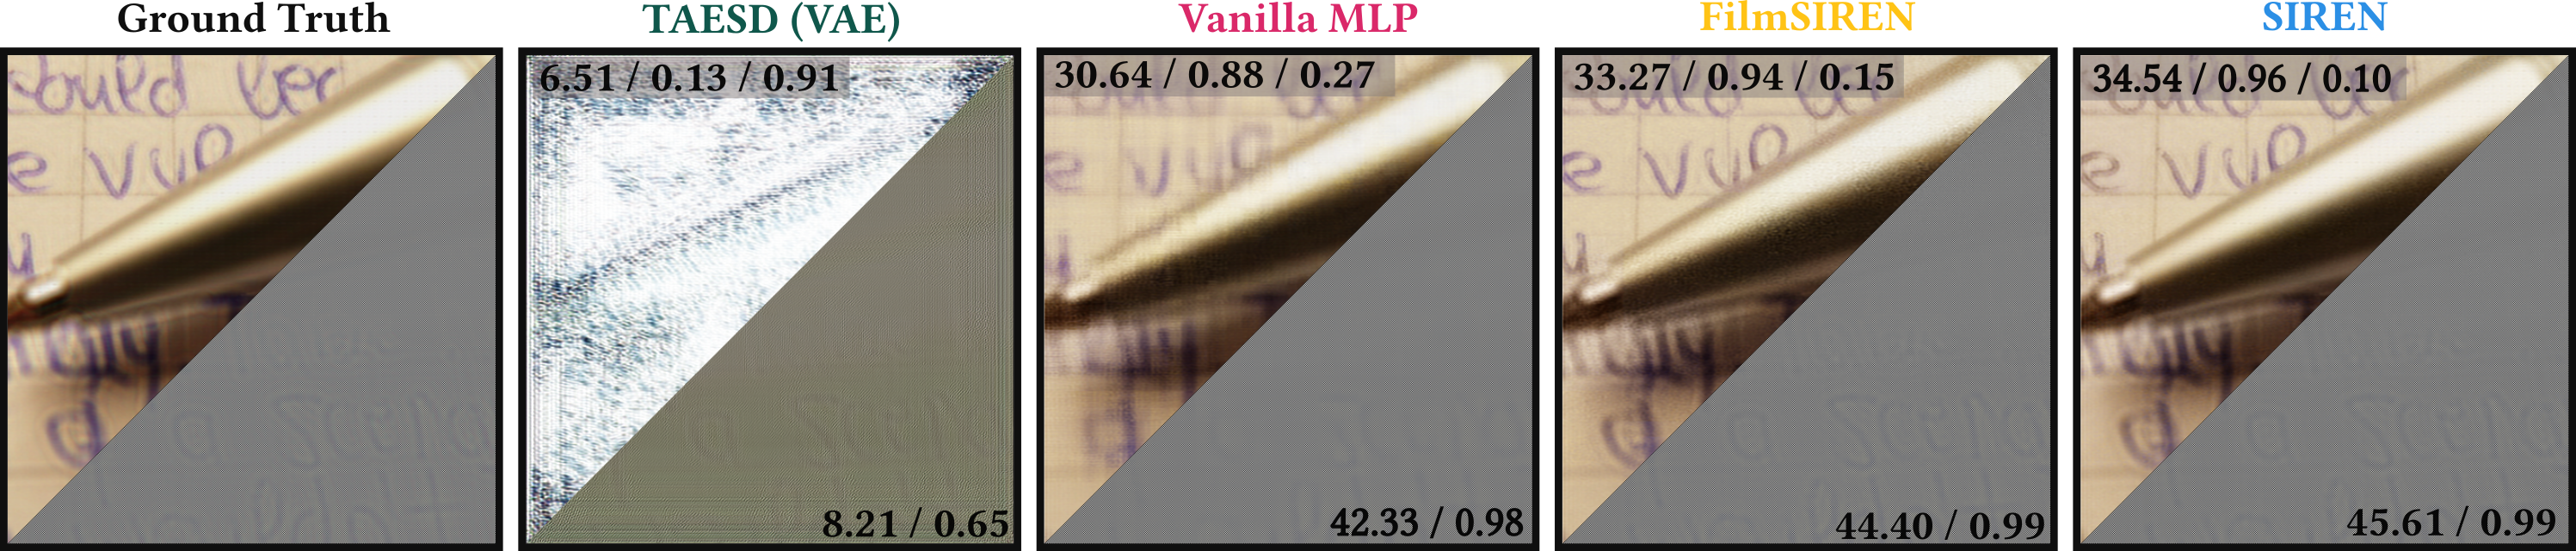
\includegraphics[width=\textwidth]{figures/teaser.png}
%   \caption{
%     example image
%     (Source image: \href{https://openverse.org/image/df8f4a77-6b7f-434f-a38a-abe5cf1f4f79?q=text&p=1}{photosteve101}).
%           }
%   \Description{}
%   \label{fig:teaser}
% \end{teaserfigure}

% \received{20 February 2007}
% \received[revised]{12 March 2009}
% \received[accepted]{5 June 2009}


\maketitle




\section{Introduction}
\section{Related works}

In the domains of augmented reality (AR) and physiological eye tracking, the extraction of deep physiological features via high-fidelity physical simulations and implicit neural representations has emerged as a critical research frontier. Recent studies have demonstrated the efficacy of computer graphics-based synthetic data in bridging the reality gap. This is achieved through the development of near-eye physical ray-tracing rendering pipelines \cite{RIT-Eyes} and 3D realistic reconstruction models equipped with relighting capabilities \cite{Realistic_nerf_eyes}.

Building upon these advancements, deep optical features---particularly Purkinje images, which encode critical information regarding crystalline lens deformation---have been leveraged alongside machine learning and miniature multi-camera arrays to achieve highly precise tracking of dynamic accommodation and vergence \cite{Dynamic_accommodation_Purkinje, Improved_vergence_and_accommodation}. However, capturing these subtle optical signals in real-world systems is frequently hindered by severe sampling noise \cite{Anti-noise_computational_imaging}. Furthermore, the downstream requirement to drive complex hardware execution mechanisms, such as variable-focus lenses \cite{Fluidic_Lenses}, necessitates a highly robust and mathematically pure underlying physical simulation framework.

To address these challenges, this paper proposes a novel framework utilizing Blender to construct a 3D anatomical eye model that supports complex refractive optical paths. By harnessing a rigorous optical rendering engine, this approach enables direct noise isolation and the precise extraction of high-dimensional deep features, including higher-order Purkinje reflections. Ultimately, this framework provides essential physical data priors for the design of next-generation, noise-robust perception networks and AR hardware systems.

\subsection{捕捉近眼图像与合成眼动追踪数据}
Recent AR depth-perception studies have used commercial eye trackers and calibrated haploscope-style optical 
setups to measure vergence responses under controlled depth changes, highlighting the need for objective and 
reproducible eye-based measurements in VAC-related experiments \cite{sturgeon2025vergence,bontha2024arhaploscope}.

Therefore, Purkinje-image-based methods seek to recover accommodation-related information from intraocular 
reflections: Lu et al. used a multi-camera, multi-LED AR-glasses prototype to track higher-order Purkinje 
images and reported a best vergence error of (0.3782^\circ) and an accommodation-depth error of 
(1.108,\mathrm{cm}) \cite{lu2020purkinje}. Ozhan et al. further combined a Purkinje imaging setup with a 
ZEMAX eye model and learning-based regression, achieving (0.17,\mathrm{D}) accommodation RMSE and (0.18^\circ) 
vergence RMSE with subject-specific data, and (0.32,\mathrm{D}) / (0.32^\circ) under leave-one-subject-out 
evaluation with two-point calibration \cite{ozhan2023dynamicaccommodation}.

These works suggest that higher-order Purkinje reflections can serve as physically meaningful cues for accommodation-aware eye tracking, 
but their weak intensity, defocus, and strong dependence on LED--camera--eye geometry make them difficult to capture robustly. Motivated by this limitation, 
we first build a controllable Blender/LuxCore optical eye model to analyze the formation, visibility, and stability of P1--P4 under near-eye infrared imaging conditions.

On the other hands, synthetic near-eye rendering provides a complementary route for studying camera--
illumination configurations: RIT-Eyes rendered three Blender/Cycles datasets with 154,800 path-traced 
near-eye images in total, including S-NVGaze, S-OpenEDS, and S-General, and evaluated SegNet and RITnet on cross-dataset eye-region segmentation, reporting a global mIoU of 86.06 
with scores ranging from 77.54 to 94.59 \cite{nair2020riteyes}. 
In addtion, EyeNeRF uses an explicit eyeball surface together with an implicit volumetric representation, 
while relightable-eye reconstruction combines an explicit cornea mesh with NeRF-style light transport 
under near-field point lights and structured illumination \cite{li2022eyenerf,khademi2026relightableeyes};


To sum up, these recent works show that both physical Purkinje tracking and synthetic eye rendering rely 
on accurate modeling of ocular geometry, illumination, and camera configuration.
 However, existing rendering or neural-representation pipelines are mainly designed for gaze estimation, 
 segmentation, or photorealistic synthesis, whereas our work focuses on physically analyzing how higher-order Purkinje images emerge under controlled near-eye IR imaging conditions.
\subsection{可重光照眼球重建与端到端物理仿真}
Excerp for physical capture, for the optical eyes modeling, the main problem including the complicated geometry of outsurface of cornea.
For example, eyenerf propose a hybrid representation, conbine explicit eyeball model to handle high-frequency high-gloss
, in the mean time, Training the Nerf model for implicit representation enables the modeling of the surrounding eye area 
and the complex appearance within the eye\cite{li2022eyenerf}. In addition, 

\textit{Reconstructing Realistic and Relightable Eyes} highlight the importance of near-field illuminationb to eyes modelling 
this use hybrid mesh + NeRF Rebuild the ocular system with reflective light capabilities and support the common near-field point lights 
and structured/fringe projectors \cite{khademi2026relightableeyes}. 

The differentiable optical design provides a reference method for optimizing the layout of LEDs, cameras and auxiliary lenses in the future of this project. \textit{End-to-end Optimization of Fluidic Lenses}
By integrating the fluid lens shape, differentiable ray tracing, and neural reconstruction into the same 
end-to-end pipeline, the loss can be back-propagated to the lens design parameters \cite{na2024fluidiclenses}. 
The work "End-to-End Hybrid Refractive-Diffractive Lens Design with Differentiable Ray-Wave Model" combines ray 
tracing and wave propagation, simultaneously simulating refractive aberrations and diffraction phase modulation, 
and supports the joint optimization of the optical system and the reconstruction network \cite{yang2024hybridlens}.
 These works illustrate that optical simulation should not merely be a post-processing tool, but can become a 
 part of the system design. Corresponding to this project, in the future, the brightness, clarity, separation 
 distance from P1, and whether it falls within the camera field of view of P3/P4 can be set as optimization 
 targets, and be used to guide the placement of LED and camera in reverse.

真实实验中，高阶 Purkinje 图像往往非常弱，尤其 P3/P4 可能受到低亮度、离焦、传感器噪声和低对比度影响。因此，
弱光图像增强和 synthetic-to-real 方法可以作为后续辅助模块。\textit{Anti-noise Computational Imaging Using 
Unsupervised Deep Learning} 说明了在缺少 clean ground truth 的情况下，也可以利用无监督深度学习改善计算成像重建质量
 \cite{zhai2022antinoise}. 扩散模型风格迁移和 physics-informed diffusion 也提供了未来方向：前者可以缩小 
 Blender/LuxCore 合成图与真实红外图像之间的 domain gap \cite{chigot2025diffusionstyletransfer}，
 后者强调生成模型应满足物理约束，而不是只追求视觉真实 \cite{bastek2025pidm}. 不过在当前阶段，核心仍应是先建立可信的 
 Blender/LuxCore 光学眼球模型，再考虑学习型增强或 domain adaptation。

 
\section{Background}

1. Blender-based Optical Eye Modeling and Purkinje Image Simulation

Purkinje images are specular reflections formed at different refractive surfaces of the eye, including the anterior and posterior corneal surfaces and the anterior and posterior crystalline lens surfaces. Compared with conventional pupil-center-corneal-reflection eye tracking, higher-order Purkinje images provide richer optical information because they are affected not only by gaze direction but also by the geometry and deformation of the crystalline lens \cite{lu2020purkinje}. This makes them especially relevant for AR/VR applications, where both vergence and accommodation are important for understanding visual comfort and accommodation--vergence conflict. However, higher-order reflections such as P3 and P4 are usually weak, defocused, and sensitive to the relative placement of the light source, camera, and eye \cite{lu2020purkinje}. Therefore, a controllable optical simulation environment is necessary before building a reliable physical capture system.

In this project, we first construct a physically interpretable eye model in Blender/LuxCore to study the formation of Purkinje images under near-eye infrared illumination. Inspired by synthetic near-eye rendering systems such as RIT-Eyes, the simulation aims to reproduce controllable near-eye image formation rather than only generate visually plausible eye images \cite{nair2020riteyes}. We explicitly model the cornea, crystalline lens, iris, and sclera, with special attention to refractive interfaces and material indices of refraction. This design is also consistent with recent relightable eye reconstruction work, where explicit eye surfaces are used to model corneal refraction and high-frequency specular reflections, while more flexible neural or volumetric representations are used for complex appearance \cite{li2022eyenerf,khademi2026relightableeyes}. Unlike avatar-oriented eye reconstruction, our simulation focuses on explaining how LED position, camera position, focal length, aperture, and optical surface geometry affect the visibility and separability of P1--P4.

2. Real Near-eye Capture with IR LED, IR Camera, and Head Stabilization

After building the simulation model, we use a real near-eye capture setup to validate whether the simulated Purkinje patterns can be observed under controlled physical conditions. The experimental setup consists of an infrared LED as the active illumination source, an IR-sensitive camera as the imaging sensor, and a headrest to stabilize the subject's head and reduce motion between the eye, camera, and light source. This physical constraint is important because Purkinje reflections are highly sensitive to small changes in geometry; even slight head movement can shift the relative positions of the cornea, crystalline lens, camera, and LED, making higher-order reflections difficult to detect consistently. Prior Purkinje-image-based AR tracking systems also emphasize that camera and LED placement must be carefully designed to capture useful higher-order reflections \cite{lu2020purkinje}.

The real capture stage is intended to complement the Blender/LuxCore simulation. The simulation provides a controlled way to test optical hypotheses, while the physical setup reveals practical issues such as sensor noise, weak reflection intensity, defocus, ambient light interference, and alignment error. These problems are especially important for P3/P4, which are much weaker than the first corneal reflection. Work on end-to-end optical design suggests that imaging hardware and computational processing should be considered jointly rather than separately \cite{na2024fluidiclenses,yang2024hybridlens}. In future extensions, the observed brightness, sharpness, and spatial separation of Purkinje images could be used as optimization targets for camera--LED placement. In addition, unsupervised anti-noise computational imaging may be useful for enhancing weak IR reflections when clean ground-truth images are unavailable \cite{zhai2022antinoise}. Thus, the proposed workflow combines physically based simulation and controlled real-world acquisition to support reliable Purkinje image analysis.
\section{Results and Discussions}
\bibliographystyle{ACM-Reference-Format}
\bibliography{references}

\end{document}